\documentclass[xcolor=dvipsnames]{beamer}
\usepackage{lmodern}
\usepackage[T1]{fontenc}
\usepackage[english]{babel}
\usepackage[utf8]{inputenc}

\usepackage{manfnt}
\usepackage{wasysym}
\usepackage{listings}
\usepackage{graphicx}
\usepackage{url}
\usepackage{ulem}
\usepackage{marvosym}
\usepackage{skull}
\usepackage{proof}
\usepackage{array}
\setbeamertemplate{navigation symbols}{}

\title[Linked Task Failure]{{\bf Parallel Programming with Failure in Rust}}
\subtitle[]{ {\em when success isn't good enough}}
\author[Ben Blum]{Ben Blum \texttt{(bblum@andrew.cmu.edu)}}

\institute[Mozilla Research]{Mozilla Research}
\date[]{2012, August 16}

\setbeamertemplate{footline}{\hspace*{.5cm}\scriptsize{\insertauthor\hspace*{50pt} \hfill\insertframenumber\hspace*{.5cm}}} 

\usecolortheme{seahorse}
\usecolortheme{rose}
\useoutertheme{infolines}

\usecolortheme[named=RoyalBlue]{structure}

\newcommand\noob{\mathsf{noob}}
\newcommand\gibs{\mathsf{gibs}}
\newcommand\dps{\mathsf{dps}}
\newcommand\squig\rightsquigarrow
\newcommand\Coloneqq{\mathrel{\mathop{::}}=}
\newcommand\dmg{\text{\Laserbeam}}
\newcommand\delter\delta
\newcommand\alpher\alpha
\newcommand\defnor{\text{ }|\text{ }}

\newcommand\pimp{\mathop{\supset}}
\newcommand\pand{\mathop{\wedge}}
\newcommand\por{\mathop{\vee}}
\newcommand\ptrue{\top}
\newcommand\pfalse{\bot}


\begin{document}
\renewcommand{\inserttotalframenumber}{28}
\normalem
\begin{frame}
	\titlepage
\end{frame}

%%%%%%%%%%%%%%%%%%%%%%%%%%%%%%%%%%%%%%%%%%%%%%%%%%%%%%%%%%%%%%%%%%%%%%%%%%%%%%%%
%%%%%%%%%%%%%%%%%%%%%%%%%%%%%%%%%%%%%%%%%%%%%%%%%%%%%%%%%%%%%%%%%%%%%%%%%%%%%%%%
%%%%%%%%%%%%%%%%%%%%%%%%%%%%%%%%%%%%%%%%%%%%%%%%%%%%%%%%%%%%%%%%%%%%%%%%%%%%%%%%

\newcommand\linegap{\vspace{0.2in}}
\newcommand\breakslide[1]{\begin{frame}{} \begin{center} \Large #1 \end{center} \end{frame}}
\newcommand\related[1]{\textsuperscript{\em [#1]}}
\newcommand\hilight[2]{\color{#1}#2\color{black}}

\begin{frame}{Outline}
	\begin{columns}[l]
	\column{0.05\textwidth}
	\column{0.5\textwidth}
	\textbf{Rustic Concurrency}
	\begin{itemize}
		\item Lightweight Tasks
		\item Communication
	\end{itemize}
	\linegap

	{\bf Motivation}
	\begin{itemize}
		\item Use Case - Writing a Browser
	\end{itemize}
	\linegap

	{\bf Failure Propagation}
	\begin{itemize}
		\item Failure-Aware Programming
		\item Failure Propagation
	\end{itemize}
	\linegap
	{\bf Extra Goodies}
	\column{0.45\textwidth}
	\begin{center}
	
\includegraphics[width=0.9\textwidth]{rust.png}
	\end{center}
	\end{columns}
\end{frame}

%%%%%%%%%%%%%%%%%%%%%%%%%%%%%%%%%%%%%%%%%%%%%%%%%%%%%%%%%%%%%%%%%%%%%%%%%%%%%%%%
\section{Rustic Concurrency}
%%%%%%%%%%%%%%%%%%%%%%%%%%%%%%%%%%%%%%%%%%%%%%%%%%%%%%%%%%%%%%%%%%%%%%%%%%%%%%%%

\newcommand\code[1]{{\begin{center}\fbox{\begin{tabular}{l} #1 \end{tabular}} \end{center}}}

\definecolor{grey}{RGB}{127,127,127}
\definecolor{darkcyan}{RGB}{0,127,127}
\definecolor{olivegreen}{RGB}{0,127,0}
\definecolor{violet}{RGB}{127,0,127}
\definecolor{brickred}{RGB}{127,0,0}
\definecolor{brown}{RGB}{127,63,0}

\subsection{Lightweight Tasks}
% slide: for 5.times println
\begin{frame}{Rust}
	A simple rust program {\small (seen at \texttt{http://rust-lang.org})}:
	\linegap
	\code{
\texttt{\hilight{brown}{fn}~\hilight{olivegreen}{main}()~\{} \\
\texttt{~~~~\hilight{brown}{for}~\hilight{brickred}{5}.times~\{} \\
%\texttt{~~~~~~~~\hilight{white}{do}~\hilight{white}{task}\hilight{white}{::spawn}~\{} \\
	\\
\texttt{~~~~~~~~~~~~\hilight{violet}{io}\hilight{grey}{::}println(\hilight{brickred}{"Here's~some~Rust!"});} \\
%\texttt{~~~~~~~~\hilight{white}{\}}} \\
\\
\texttt{~~~~\}} \\
\texttt{\}} \\
	}
\end{frame}
%		fn main() {
%		    for 5.times {
%		        io::println("Here's some Rust!");
%		    }
%		}
% slide: for 5.times task spawn println
\begin{frame}{Parallel Rust}
	The same rust program, made parallel: {\small \hilight{white}{(seen at \texttt{http://rust-lang.org})}}
	\linegap
	\code{
\texttt{\hilight{brown}{fn}~\hilight{olivegreen}{main}()~\{} \\
\texttt{~~~~\hilight{brown}{for}~\hilight{brickred}{5}.times~\{} \\
\texttt{~~~~~~~~\hilight{brown}{do}~\hilight{violet}{task}\hilight{grey}{::}spawn~\{} \\
\texttt{~~~~~~~~~~~~\hilight{violet}{io}\hilight{grey}{::}println(\hilight{brickred}{"Here's~some~Rust!"});} \\
\texttt{~~~~~~~~\}} \\
\texttt{~~~~\}} \\
\texttt{\}} \\
	}
\end{frame}
%		fn main() {
%		    for 5.times {
%		        do task::spawn {
%		            io::println("Here's some Rust!");
%		        }
%		    }
%		}

\subsection{Communication}
% slide: pipes, uniques, surrender ownership
\begin{frame}{Rust's Memory Model}
	No shared state between tasks! \\
	\code {
\texttt{\hilight{brown}{fn}~\hilight{olivegreen}{main}()~\{} \\
\texttt{~~~~\hilight{brown}{let}~\hilight{brown}{mut}~state~=~0;} \\
\texttt{~~~~\hilight{brown}{let}~state\_ptr~=~\&\hilight{brown}{mut}~state;} \\
\texttt{~~~~\hilight{brown}{do}~\hilight{violet}{task}\hilight{grey}{::}spawn~\{} \\
\texttt{~~~~~~~~*state\_ptr~+=~1;} \\
\texttt{~~~~\}} \\
\texttt{~~~~\hilight{blue}{debug!}(\hilight{brickred}{"\%d"},~state);} \\
\texttt{\}} \\
	}
	Fails to compile:
	\begin{center} \begin{tabular}{l}
		\texttt{\hilight{red}{error:}~not a sendable value} \\
		\texttt{*state\_ptr += 1;} \\
		\texttt{~\^{}\textasciitilde\textasciitilde\textasciitilde\textasciitilde\textasciitilde\textasciitilde\textasciitilde\textasciitilde}
	\end{tabular} \end{center}
\end{frame}
%fn main() {
%    let mut state = 0;
%    let state_ptr = &mut state;
%    do task::spawn {
%        *state_ptr += 1;
%    }
%    debug!("%d", state);
%}

\begin{frame}{Communication with Message Passing}
	Message passing
	\begin{itemize}
		\item Send and receive on pipes
		\item Sending state means giving up ownership
	\end{itemize}
	\linegap
	\code{
		\\
\texttt{\hilight{brown}{let}~(sender,~receiver)~=~\hilight{violet}{pipes}\hilight{grey}{::}stream();} \\
\texttt{\hilight{violet}{task}\hilight{grey}{::}spawn(child\_fn(receiver));} \\
\texttt{sender.send(\textasciitilde\hilight{brickred}{"Hello~world!"});} \\
\\
	}
%		let (sender, receiver) = pipes::stream();
%		task::spawn(child_fn(receiver));
%		sender.send(~"Hello world!");
\end{frame}

%%%%%%%%%%%%%%%%%%%%%%%%%%%%%%%%%%%%%%%%%%%%%%%%%%%%%%%%%%%%%%%%%%%%%%%%%%%%%%%%
\section{Motivation}
%%%%%%%%%%%%%%%%%%%%%%%%%%%%%%%%%%%%%%%%%%%%%%%%%%%%%%%%%%%%%%%%%%%%%%%%%%%%%%%%

\breakslide{What if we wrote a web browser in Rust?}

\subsection{Use Cases}
% slide: browser image rendering
\begin{frame}{Parallel Rendering}
	\begin{itemize}
		\item Webpages have many different elements.
		\item Why not wait on multiple network connections at once?
	\end{itemize}
	\linegap
	\begin{center}
	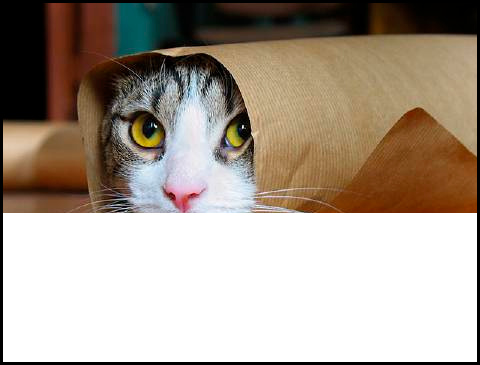
\includegraphics[width=0.25\textwidth]{burrito-2.jpg}
	\hspace{0.05\textwidth}
	
\includegraphics[width=0.25\textwidth]{burrito-3.jpg}
	\hspace{0.05\textwidth}
	
\includegraphics[width=0.25\textwidth]{burrito-1.jpg}
	\end{center}
\end{frame}
% slide: pipelined parsing/lexing HTML and CSS
\begin{frame}{Pipelined HTML/CSS Decoding}
	\begin{itemize}
		\item Coming up in Servo
		\item Lexer processes parser's output before parser finishes
	\end{itemize}
	\linegap
	\begin{center}
	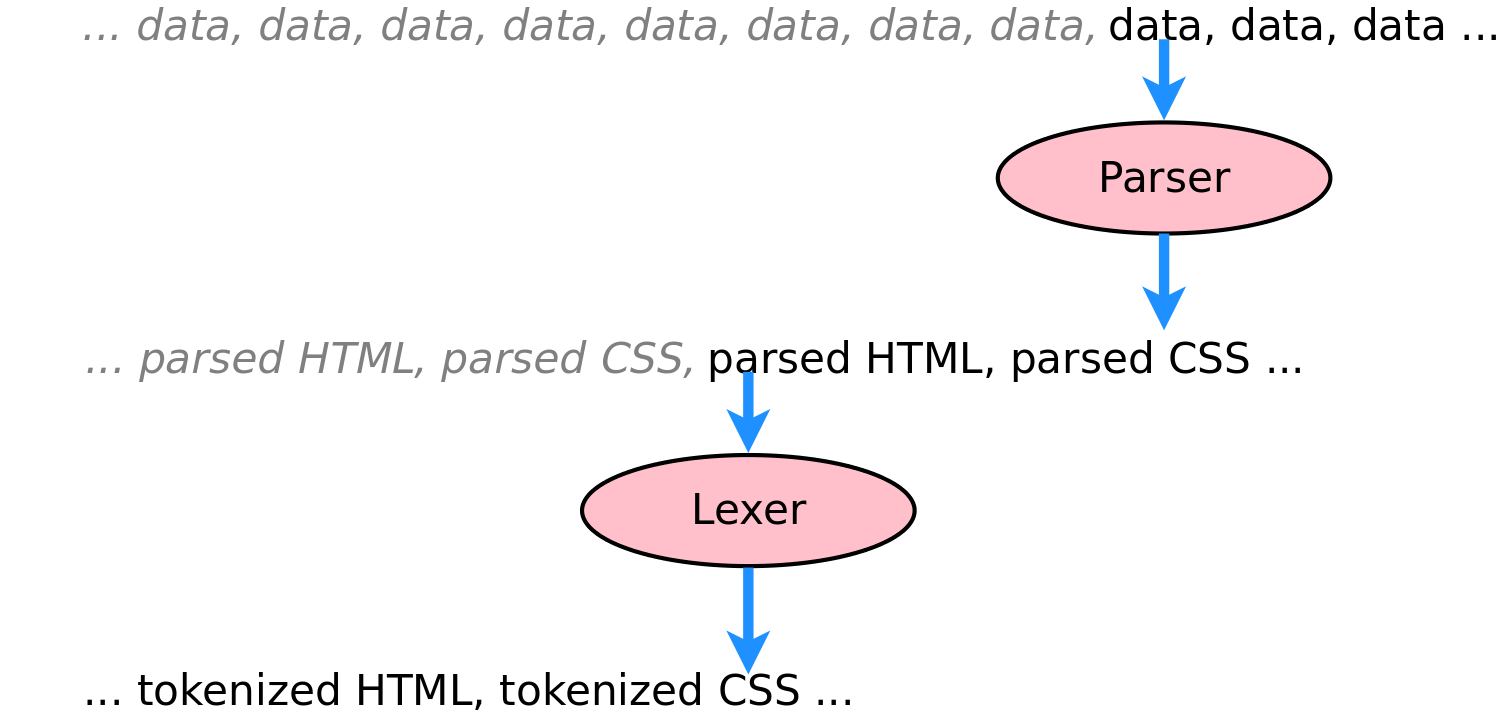
\includegraphics[width=0.8\textwidth]{parselex.png}
	\end{center}
\end{frame}
% slide: each tab is unlinked from each other
\begin{frame}{Isolated Tabs}
	\begin{center}
	
\includegraphics[width=0.75\textwidth]{manytabs.png}
	\end{center}
\end{frame}

%%%%%%%%%%%%%%%%%%%%%%%%%%%%%%%%%%%%%%%%%%%%%%%%%%%%%%%%%%%%%%%%%%%%%%%%%%%%%%%%
\section{Failure Propagation}
%%%%%%%%%%%%%%%%%%%%%%%%%%%%%%%%%%%%%%%%%%%%%%%%%%%%%%%%%%%%%%%%%%%%%%%%%%%%%%%%

\subsection{Types of Failure}

\breakslide{When things go wrong\dots}

\begin{frame}{Types of Failure}
	Different types of failure need to be handled differently.
	\begin{itemize}
		\item User abort (e.g. closing a tab)
		\item Logic error (an assert trips)
		\item Malformed input
		\item Bug in other software (graphics drivers)
	\end{itemize}
\end{frame}

\subsection{Failure-Aware Programming}

\begin{frame}{Using Linked Failure}
	Rust tasks have three main spawn modes.
	\begin{itemize}
		\item \texttt{\hilight{violet}{task}\hilight{grey}{::}spawn\_supervised()}
		\begin{itemize}
			\item Parent task failure propagates to children
		\end{itemize}
		\item \texttt{\hilight{violet}{task}\hilight{grey}{::}spawn\_linked()}
		\begin{itemize}
			\item Tasks in a ``linked failure group''
		\end{itemize}
		\item \texttt{\hilight{violet}{task}\hilight{grey}{::}spawn\_unlinked()}
		\begin{itemize}
			\item Tasks with isolated failure
		\end{itemize}
	\end{itemize}
	\linegap
	\texttt{\hilight{violet}{task}\hilight{grey}{::}spawn()} is equivalent to \texttt{spawn\_linked()}.
\end{frame}

\subsection{Directions}
% slide: two directions of rendering failure (punt image threads awake from network)
\begin{frame}{Unidirectional Failure}
	\begin{itemize}
		\item {\bf ``Supervised'' tasks:} one task is in charge of several children.
	\end{itemize}
	\begin{center}
	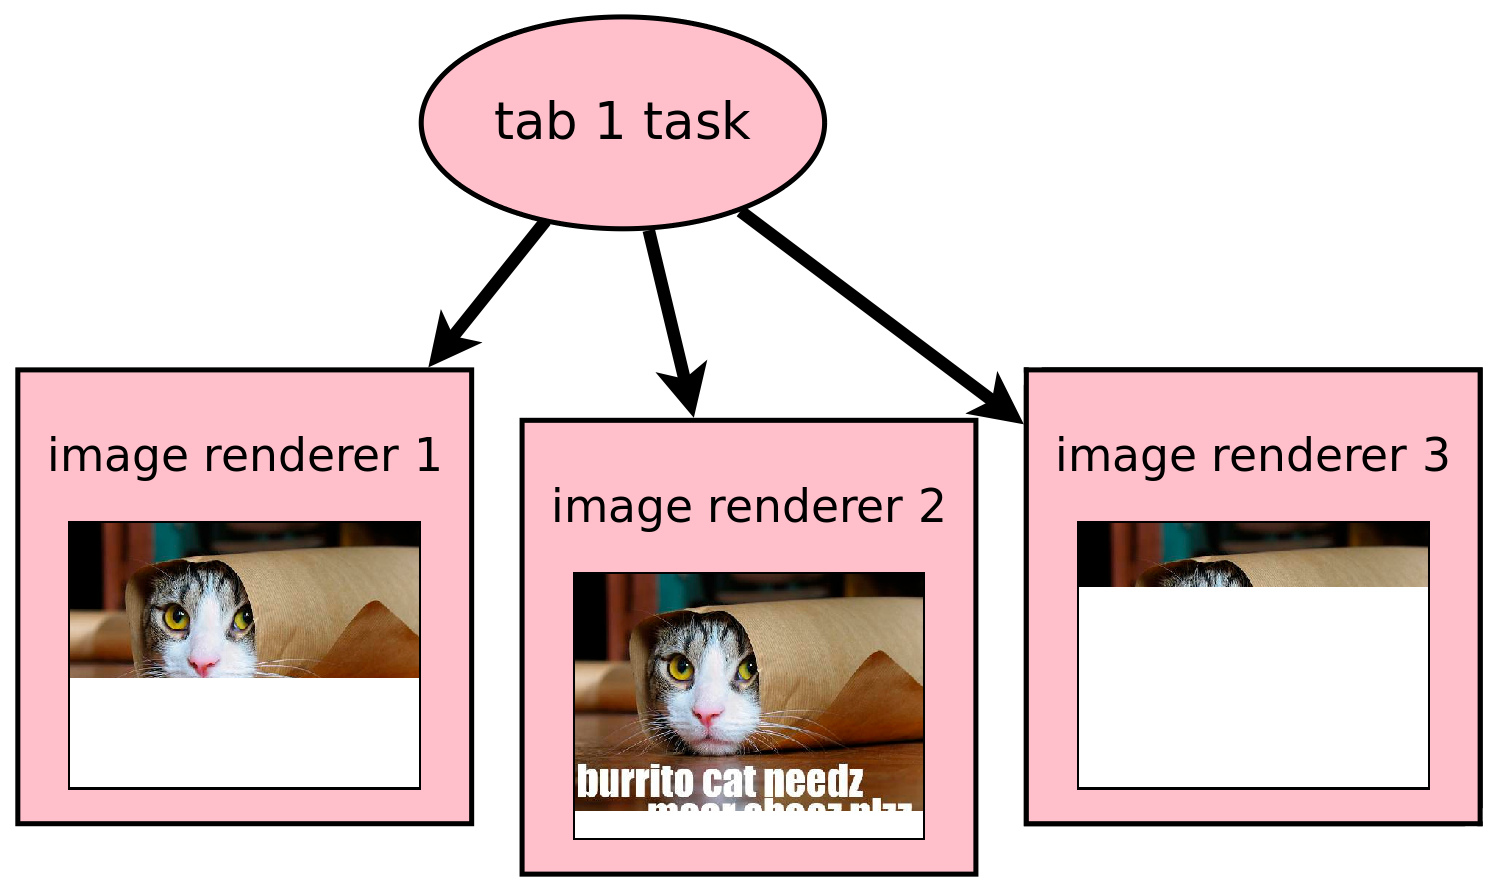
\includegraphics[width=0.7\textwidth]{unidirectional.png}
	\end{center}
\end{frame}
\begin{frame}{Unidirectional Failure}
	\begin{itemize}
		\item Child task failure should not take out the parent\dots
	\end{itemize}
	\begin{center}
	\includegraphics[width=0.7\textwidth]{unidirectional-4.png}
	\end{center}
\end{frame}
\begin{frame}{Unidirectional Failure}
	\begin{itemize}
		\item \dots but if the parent task fails,
	\end{itemize}
	\begin{center}
	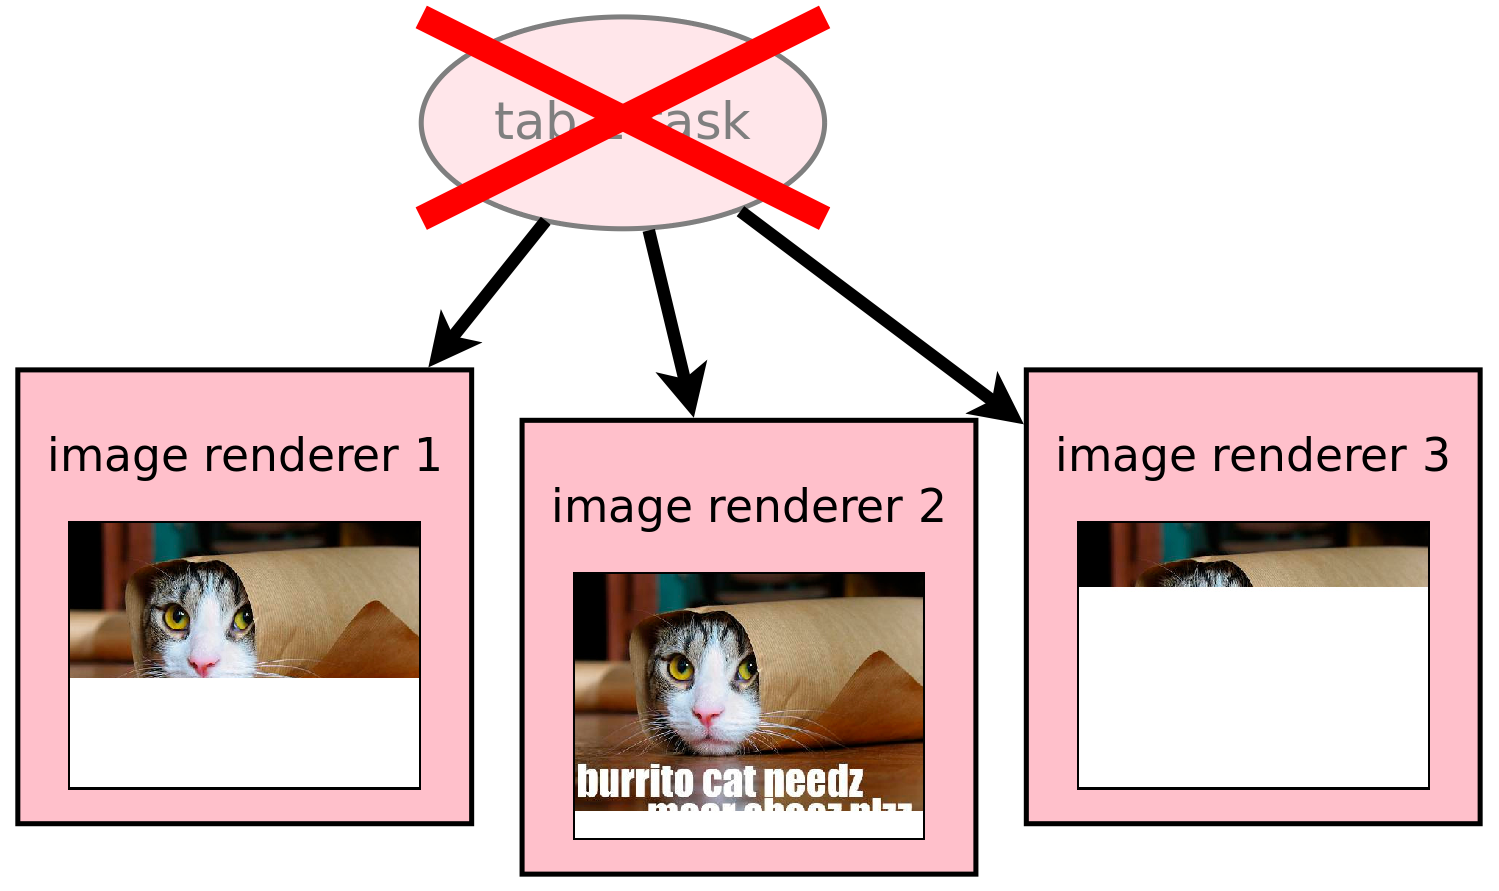
\includegraphics[width=0.7\textwidth]{unidirectional-2.png}
	\end{center}
\end{frame}
\begin{frame}{Unidirectional Failure}
	\begin{itemize}
		\item \dots but if the parent task fails, its children should die too
	\end{itemize}
	\begin{center}
	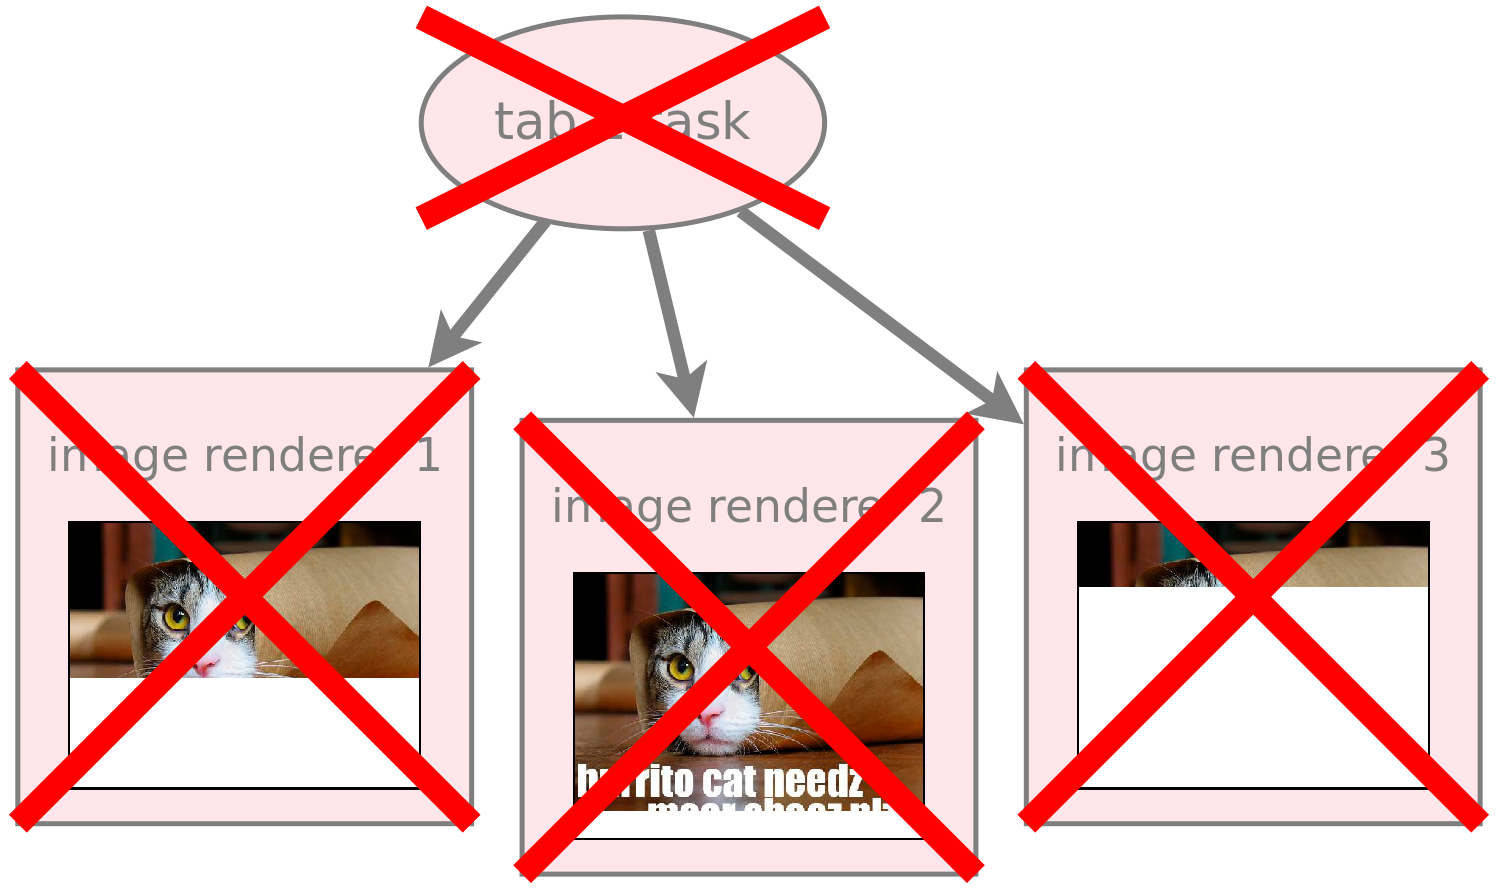
\includegraphics[width=0.7\textwidth]{unidirectional-3.png}
	\end{center}
\end{frame}
% slide: lexer and parser are able t kill each other
\begin{frame}{Bidirectional Failure}
	\begin{itemize}
		\item {\bf ``Linked'' tasks:} if either task fails, all others are killed.
	\end{itemize}
	\begin{center}
	\includegraphics[width=0.8\textwidth]{parselex-1.png}
	\end{center}
\end{frame}
\begin{frame}{Bidirectional Failure}
	\begin{itemize}
		\item If the parser finds invalid input, the lexer should die too,
	\end{itemize}
	\begin{center}
	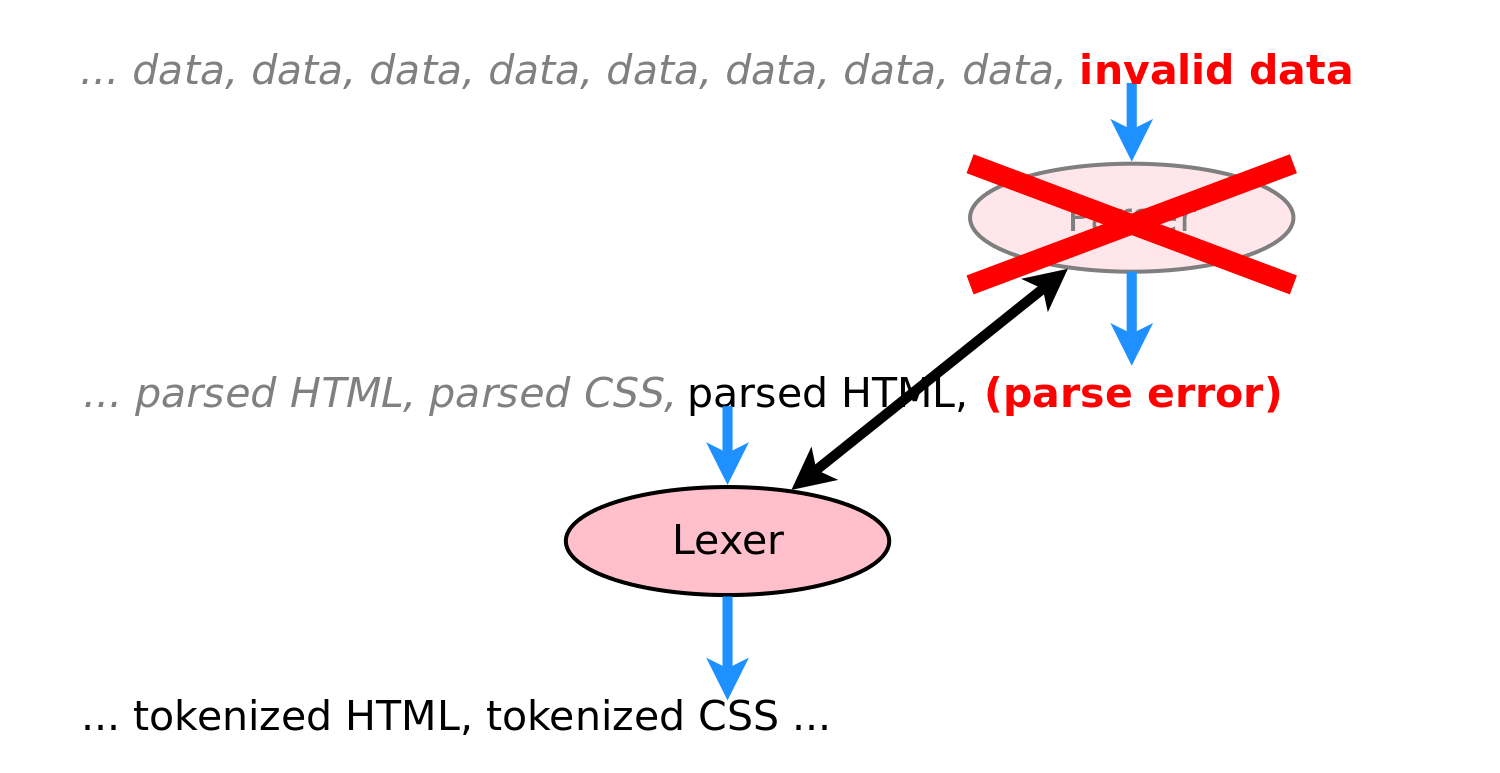
\includegraphics[width=0.8\textwidth]{parselex-2.png}
	\end{center}
\end{frame}
\begin{frame}{Bidirectional Failure}
	\begin{itemize}
		\item If the parser finds invalid input, the lexer should die too,
	\end{itemize}
	\begin{center}
	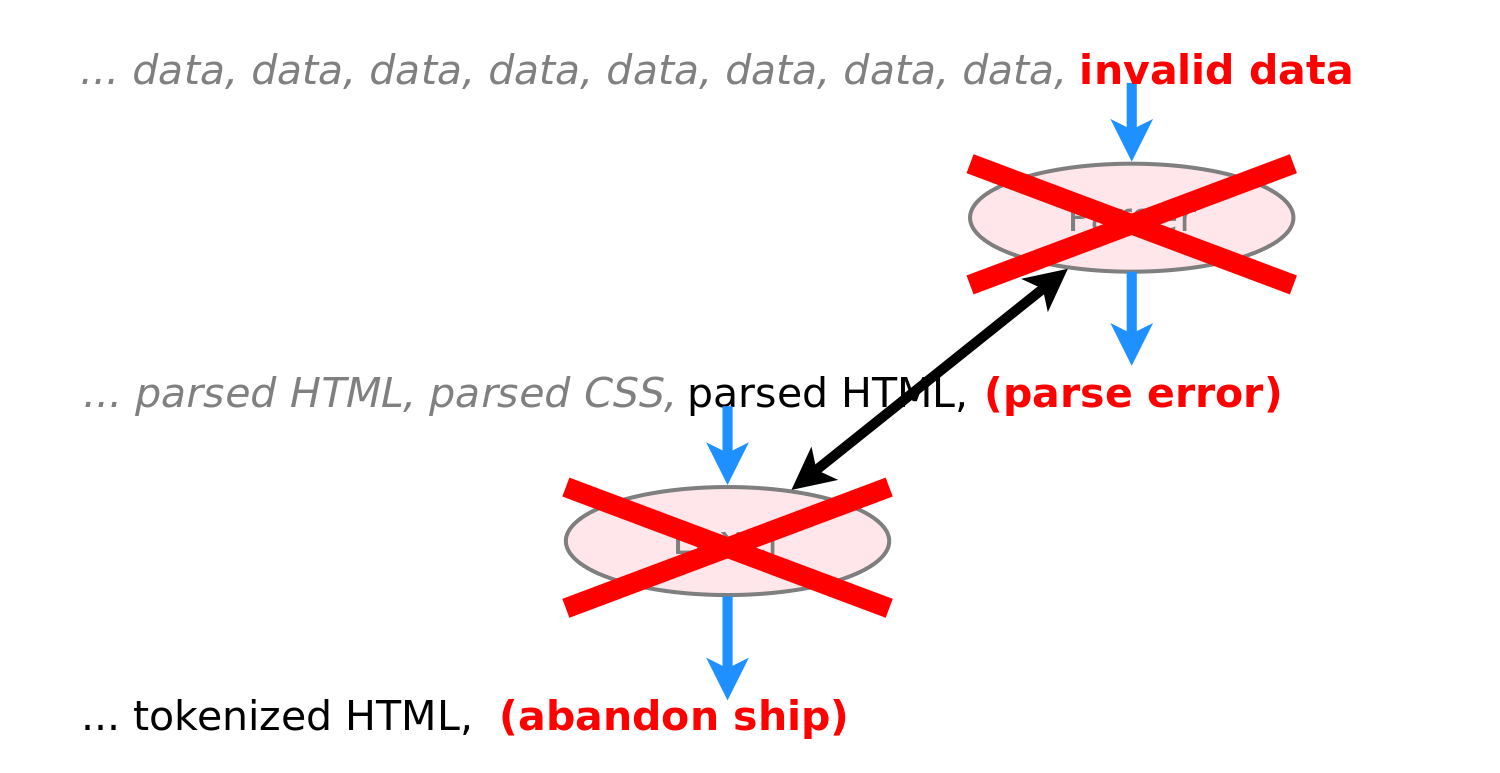
\includegraphics[width=0.8\textwidth]{parselex-3.png}
	\end{center}
\end{frame}
\begin{frame}{Bidirectional Failure}
	\begin{itemize}
		\item \dots and if the lexer has a problem, the parser should also stop.
	\end{itemize}
	\begin{center}
	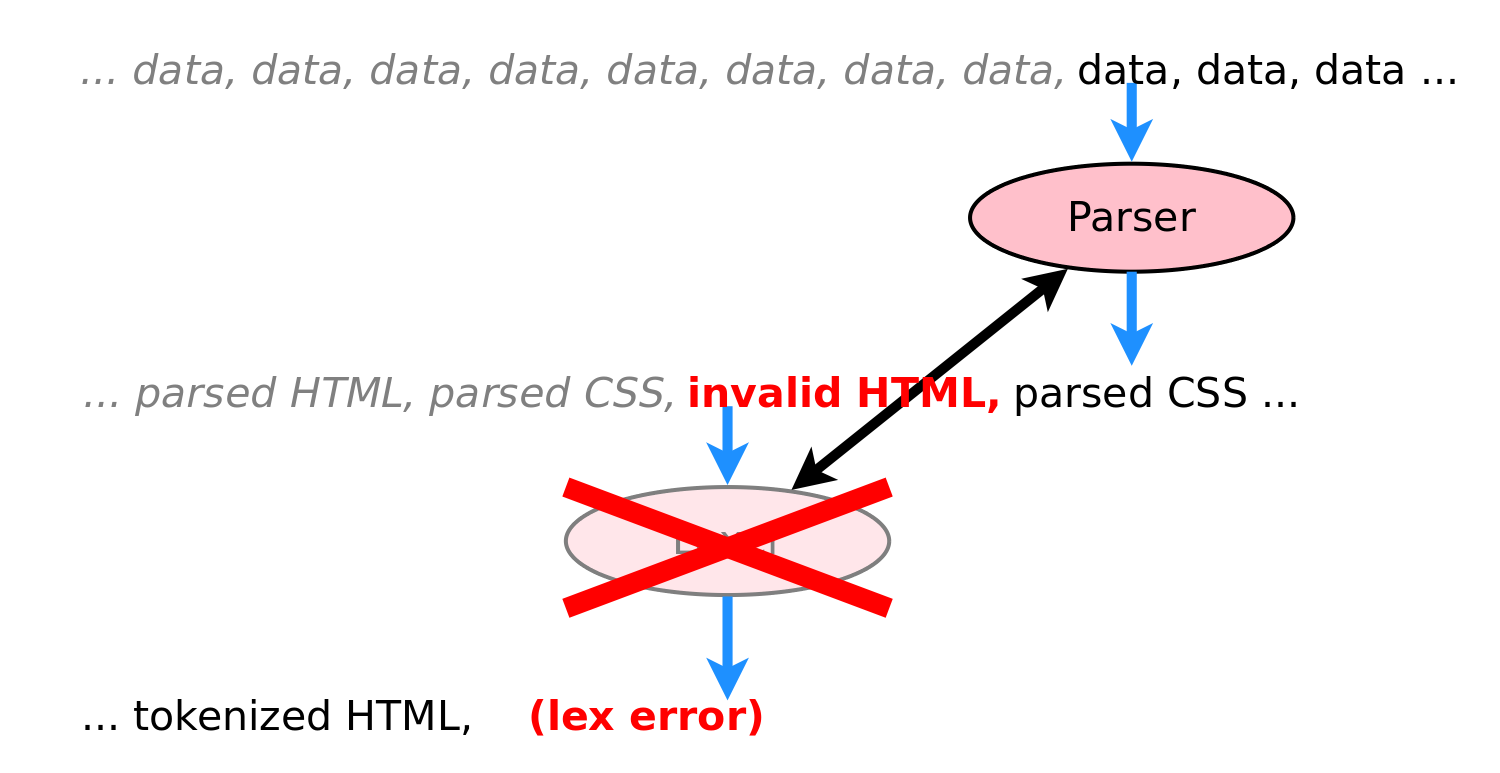
\includegraphics[width=0.8\textwidth]{parselex-4.png}
	\end{center}
\end{frame}
\begin{frame}{Bidirectional Failure}
	\begin{itemize}
		\item \dots and if the lexer has a problem, the parser should also stop.
	\end{itemize}
	\begin{center}
	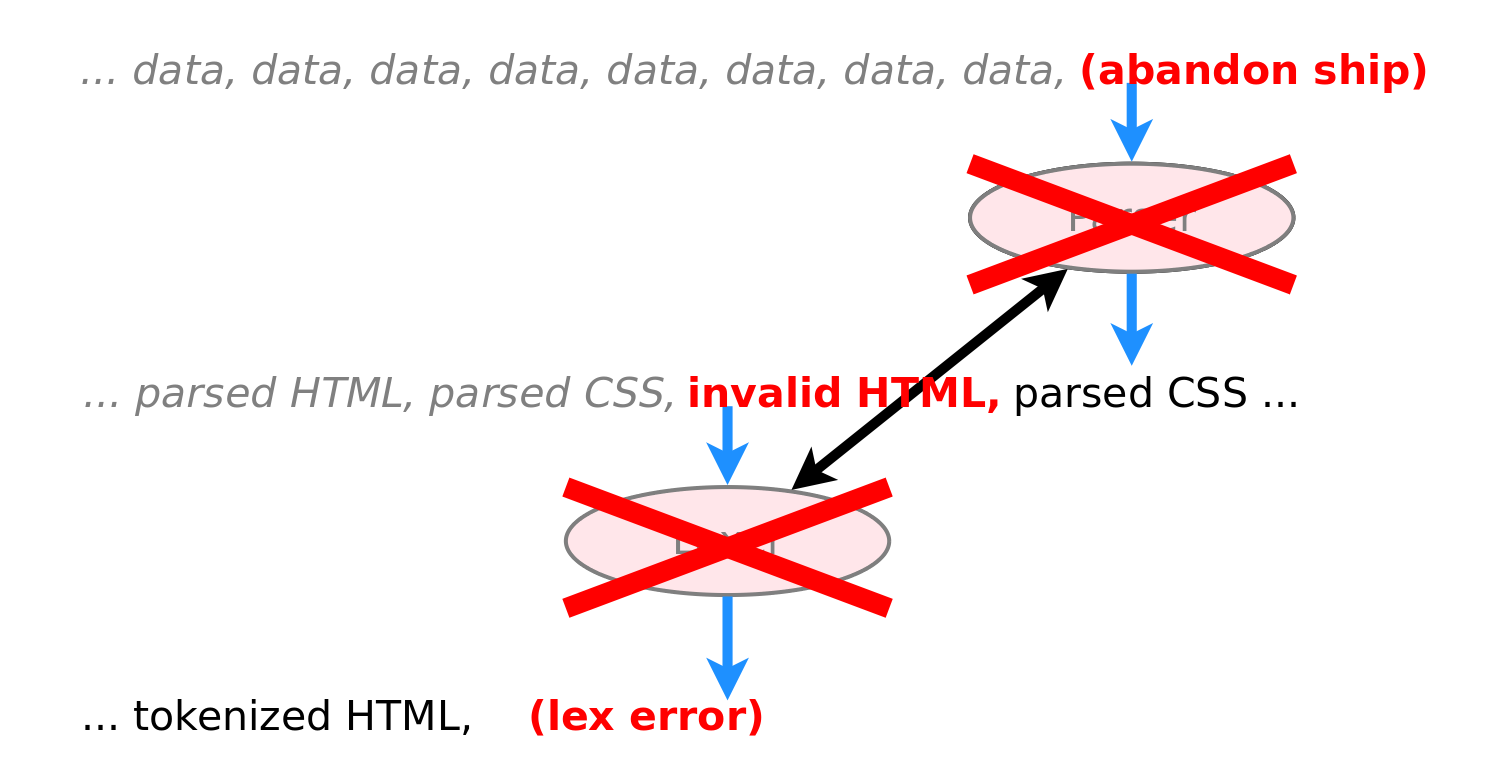
\includegraphics[width=0.8\textwidth]{parselex-5.png}
	\end{center}
\end{frame}
% slide: a tab crashes
\begin{frame}{Isolated Failure}
	\begin{itemize}
		\item {\bf ``Unlinked'' tasks:} a task's failure does not affect any other task.
	\end{itemize}
	\begin{center}
	
\includegraphics[width=0.7\textwidth]{embarrassing-blank.png}
	\end{center}
\end{frame}
\begin{frame}{Isolated Failure}
	\begin{itemize}
		\item {\bf ``Unlinked'' tasks:} a task's failure does not affect any other task.
	\end{itemize}
	\begin{center}
	\includegraphics[width=0.7\textwidth]{embarrassing.png}
	\end{center}
\end{frame}

%%%%%%%%%%%%%%%%%%%%%%%%%%%%%%%%%%%%%%%%%%%%%%%%%%%%%%%%%%%%%%%%%%%%%%%%%%%%%%%%
\section{Extra Goodies}
%%%%%%%%%%%%%%%%%%%%%%%%%%%%%%%%%%%%%%%%%%%%%%%%%%%%%%%%%%%%%%%%%%%%%%%%%%%%%%%%

\breakslide{More fun with tasks}

%\begin{frame}{Waiting for tasks}
%	\texttt{\hilight{violet}{task}\hilight{grey}{::}try()}
%	\begin{itemize}
%		\item Spawns a supervised task and waits for it to finish.
%	\end{itemize}
%			\code {
%\texttt{\hilight{brown}{let}~result~=~\hilight{violet}{task}\hilight{grey}{::}try(risky\_operation);} \\
%\texttt{\hilight{red}{assert}~result.is\_success();} \\
%			}
%%				let result = task::try(risky_operation);
%%				assert result.is_success();
%	\linegap
%	\texttt{\hilight{violet}{future}\hilight{grey}{::}get()}
%	\begin{itemize}
%		\item Can spawn many tasks and wait on them later.
%	\end{itemize}
%\end{frame}
\begin{frame}{Advanced Spawn Options}
	\texttt{\hilight{violet}{task}\hilight{grey}{::}task().foo(x).bar(y).baz(z).spawn} \dots
	\linegap
	\begin{itemize}
		\item \texttt{unlinked()}, \texttt{supervised()}, \texttt{linked()}
		\item \texttt{sched\_mode()} - configure the scheduler (N:M, N:N, N:1)
		\item \texttt{future\_result()} - lets you block on the task later
		\item \texttt{try()} - waits and gives a success/failure result
		\item \texttt{spawn\_conversation()} - sets up pipes between the tasks
	\end{itemize}
\end{frame}
%%%%%%%%%%%%%%%%%%%%%%%%%%%%%%%%%%%%%%%%%%%%%%%%%%%%%%%%%%%%%%%%%%%%%%%%%%%%%%%%
\section{Conclusion}
%%%%%%%%%%%%%%%%%%%%%%%%%%%%%%%%%%%%%%%%%%%%%%%%%%%%%%%%%%%%%%%%%%%%%%%%%%%%%%%%

\breakslide{Thanks to\dots}

\begin{frame}{Questions?}
	% rust logo
	\begin{center}
		
\includegraphics[width=0.6\textwidth]{rust.png}
	\end{center}
\end{frame}

\begin{frame}{Bonus slides}
	\begin{center}
	\large \textit{(I'm glad you asked that\dots)}
	\end{center}
\end{frame}
\begin{frame}{Upwards failure propagation}
	\code{
\texttt{\hilight{brown}{do}~\hilight{violet}{task}\hilight{grey}{::}spawn~\{~\hilight{darkcyan}{//~linked}} \\
\texttt{~~~~\hilight{brown}{let}~result~=~\hilight{brown}{do}~\hilight{violet}{task}\hilight{grey}{::}task().unlinked().try~\{} \\
\texttt{~~~~~~~~\hilight{darkcyan}{//~...~if~i~fail,~the~parent~dies,}} \\
\texttt{~~~~~~~~\hilight{darkcyan}{//~~~~~but~the~parent~can't~kill~me~...}} \\
\texttt{~~~~\}} \\
\texttt{~~~~\hilight{brown}{if}~result.is\_err()~\{} \\
	\texttt{~~~~~~~~\hilight{red}{fail}~\textasciitilde\hilight{brickred}{"Child~failed"}~\hilight{darkcyan}{//~linked~to~original~task}} \\
\texttt{~~~~\}} \\
\texttt{\}} \\
	}
%		do task::spawn { // linked
%		    let result = do task::task().unlinked().try {
%		        // ... if i fail, the parent dies,
%		        //     but the parent can't kill me ...
%		    }
%		    if result.is_err() {
%		        fail ~"Child failed" // linked to original task
%		    }
%		}
\end{frame}

\begin{frame}{Hardest Part}
	Unidirectional failure across multiple generations
	\code{
\texttt{\hilight{brown}{do}~\hilight{violet}{task}\hilight{grey}{::}spawn\_supervised~\{} \\
\texttt{~~~~\hilight{brown}{do}~\hilight{violet}{task}\hilight{grey}{::}spawn\_supervised~\{} \\
\texttt{~~~~~~~~\hilight{darkcyan}{//~Grandchild~task~blocks~forever}} \\
\texttt{~~~~~~~~port.recv();} \\
\texttt{~~~~\}} \\
\texttt{~~~~\hilight{darkcyan}{//~Middle~task~exits~early}} \\
\texttt{\}} \\
\texttt{\hilight{red}{fail};~\hilight{darkcyan}{//~Must~kill~grandchild~task}} \\
	}
%		do task::spawn_supervised {
%		    do task::spawn_supervised {
%		        // Grandchild task blocks forever
%		        port.recv();
%		    }
%		    // Middle task exits early
%		}
%		fail; // Must kill grandchild task
\end{frame}
\begin{frame}{Hardest Part}
	Unidirectional failure across multiple generations
	\begin{center}
	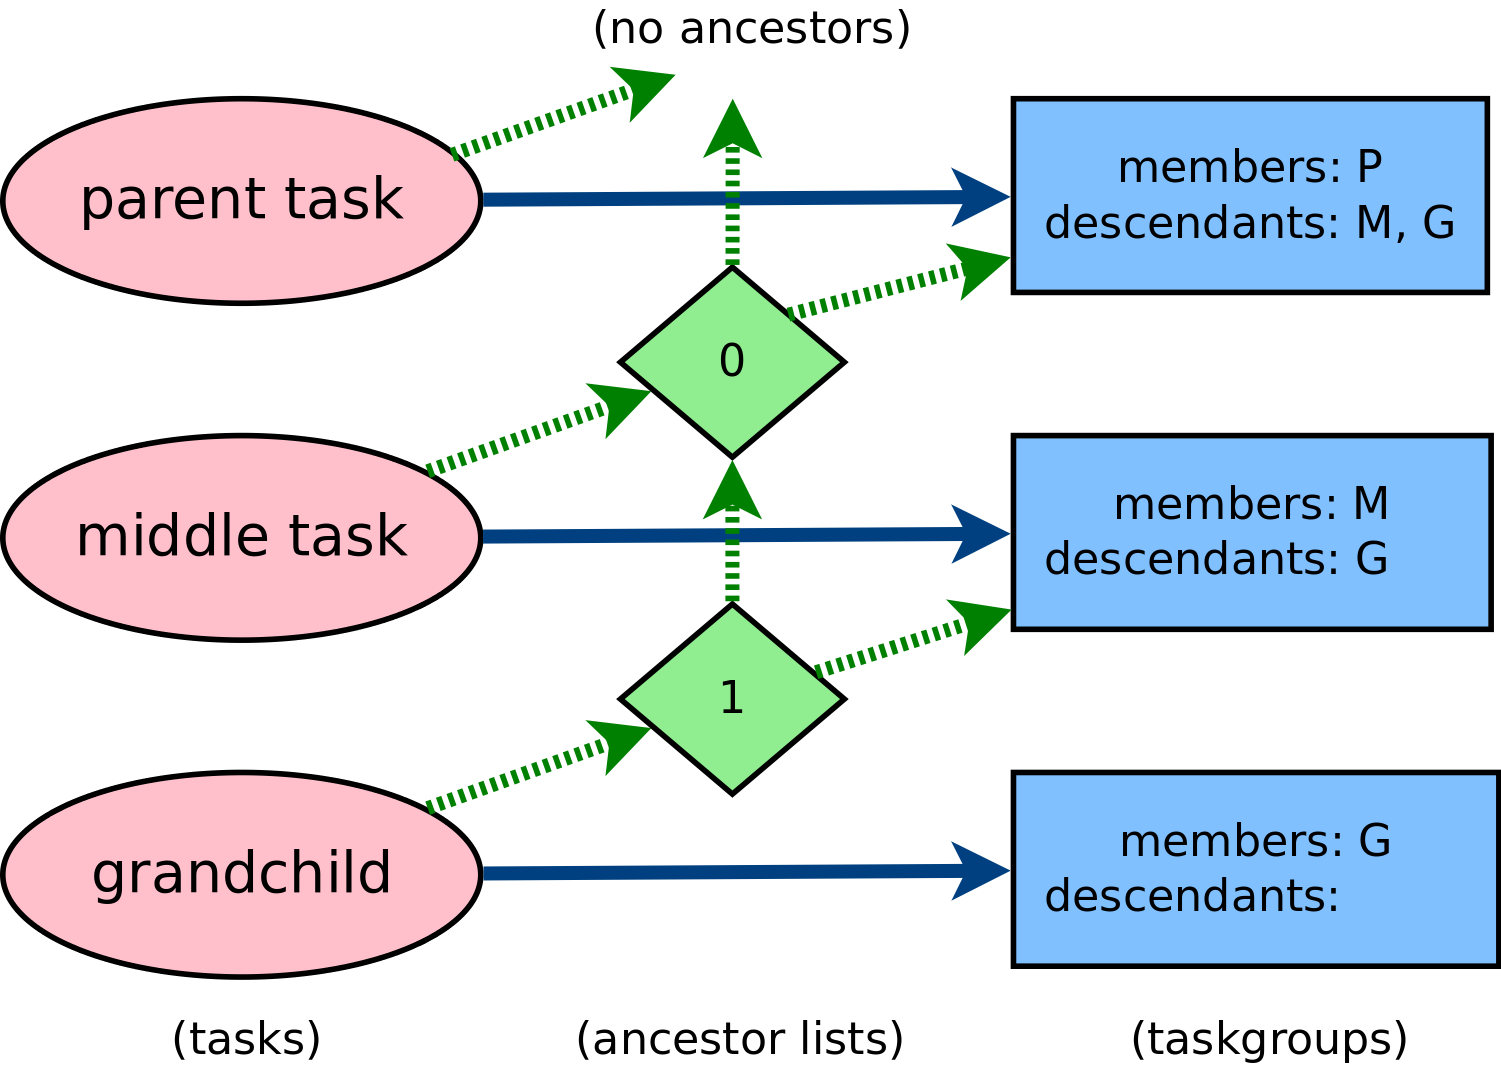
\includegraphics[width=0.7\textwidth]{ancestors.png}
	\end{center}
\end{frame}

\begin{frame}{Concurrency Primitives and Shared State}
	\textbf{``RW-ARC'':} reader-/writer-locked atomically-refcounted shared state.
	\code {
		\texttt{\hilight{brown}{impl}~<T:~\hilight{brown}{const}~\hilight{brown}{send}>~\&\hilight{olivegreen}{rw\_arc}<T>~\{} \\
\texttt{~~~~\hilight{brown}{fn}~\hilight{olivegreen}{read}~~~~~~(blk:~\hilight{brown}{fn}(\&T));} \\
\texttt{~~~~\hilight{brown}{fn}~\hilight{olivegreen}{write}~~~~~(blk:~\hilight{brown}{fn}(\&\hilight{brown}{mut}~T));} \\
\texttt{~~~~\hilight{brown}{fn}~\hilight{olivegreen}{write\_cond}(blk:~\hilight{brown}{fn}(\&\hilight{brown}{mut}~T,~\&condvar));} \\
\texttt{\}} \\
	}
%		impl <T: const send> &rw_arc<T> {
%		    fn read      (blk: fn(&T));
%		    fn write     (blk: fn(&mut T));
%		    fn write_cond(blk: fn(&mut T, &condvar));
%		}

	\begin{center}
	\begin{tabular}{cc}
		\begin{tabular}{l}
\texttt{\hilight{brown}{do}~arc.write\_cond~|state,c|~\{} \\
\texttt{~~~~\hilight{darkcyan}{//~exclusive~access}} \\
\texttt{~~~~c.wait();} \\
\texttt{~~~~\hilight{darkcyan}{//~can~modify~the~data}} \\
\texttt{~~~~*state~=~\hilight{brickred}{17};} \\
\texttt{~~~~c.signal();} \\
\texttt{\}} \\
		\end{tabular}
	&
%		do arc.write_cond |state, cond| {
%		    // exclusive access
%		    cond.wait();    // can block...
%		    *state = 17;    // modify the data...
%		    cond.signal();  // and wake others
%		}
		\begin{tabular}{l}
\texttt{\hilight{brown}{do}~arc.read~|state|~\{} \\
\texttt{~~~~\hilight{darkcyan}{//~concurrent~access}} \\
\texttt{~~~~\hilight{darkcyan}{//~immutable~state}} \\
\texttt{~~~~\hilight{red}{assert}~*state~==~\hilight{brickred}{17};} \\
\texttt{~~~~\hilight{darkcyan}{//~Won't~compile}} \\
\texttt{~~~~*state~+=~\hilight{brickred}{1};} \\
\texttt{\}} \\
		\end{tabular}
	\end{tabular}
	\end{center}
%		do arc.read |state| {
%		    // shared access - immutable state
%		    assert *state == 17;  // OK
%		    *state += 1;  // Won't compile
%		}
\end{frame}


\end{document}

%%%%%%%%%%%%%%%%%%%%%%%%%%%%%%%%%%%%%%%%%%%%%%%%%%%%%%%%%%%%%%%%%%%%%%%%%%%%%%%%
% vim: foldmethod=indent
